%
\chapter{Elektronski sistemi določanja lastnega položaja}
\label{Ch:ElSistLastPoloz} % Always give a unique label
% use \chaptermark{}
% to alter or adjust the chapter heading in the running head
Določanje položaja smo orisali že v uvodnem poglavju \ref{SubSec:TehnDolPoloz}. Ko določamo ali svoj lastni položaj ali položaj drugega objekta v prostoru, je vedno potrebno definirati čas in koordinatni sistem, v katerem podajamo položaj. Poznati moramo izhodišče koordinatnega sistema, usmerjenost koordinatnih osi in enote. 

Mednarodna pomorska organizacija je svojo iniciativo za usklajeno zbiranje, vključevanje, izmenjavo, predstavljanje in analizo pomorskih informacij na ladji poimenovala e-navigacija. Z omenjeno inciativo želi IMO v duhu sednjega časa poživiti navigacijo od priveza do priveza in vse z njo povezane storitve, ki zagotavljajo varnost in zaščito na morju ter varovanje pomorskega okolja. Princip e-navigacije predvideva, da se mora za določanje časa in položaja uporabljati dva različna in med seboj neodvisna vira podatkov, da bo dobljeni sistem trpežen in da v primeru odpovedi enega dela preostali deli ohranijo funkcijo celotnega sistema.

%ČAS za definiranje časa potrebujemo oscilator za določitev koliko nihajev spravimo v eno časovno enoto in določitev izhodišča 
% http://www.ieee-uffc.org/frequency-control/learning-vig.asp?chapter=vigintro
% More than one billion (i.e., 109) quartz crystal oscillators are produced annually for applications ranging from inexpensive watches and clocks to radionavigation and spacecraft tracking systems. The fundamentals of quartz oscillators are reviewed in this report, with emphasis on quartz frequency standards (as opposed to inexpensive clock oscillators). The subjects discussed include: crystal resonators and oscillators, oscillator types, and the characteristics and limitations of temperature-compensated crystal oscillators (TCXO) and oven-controlled crystal oscillators (OCXO). The oscillator instabilities discussed include: aging, noise, frequency vs. temperature, warmup, acceleration effects, magnetic field effects, atmospheric pressure effects, radiation effects, and interactions among the various effects. Guidelines are provided for oscillator comparison and selection. Discussions of specifications are also included, as are references and suggestions for further reading.
% Figure 1 is a greatly simplified circuit diagram that shows the basic elements of a crystal oscillator [1-3]. The amplifier of a crystal oscillator consists of at least one active device, the necessary biasing networks; and may include other elements for band limiting, impedance matching, and gain control. The feedback network consists of the crystal resonator, and may contain other elements, such as a variable capacitor for tuning.

%Figure 1 
%Figure 1. Crystal Oscillator - simplified circuit diagram.
%
%The frequency of oscillation is determined by the requirement that the closed loop phase shift = 2np, where n is an integer, usually 0 or 1. When the oscillator is initially energized, the only signal in the circuit is noise. That component of noise, the frequency of which satisfies the phase condition for oscillation, is propagated around the loop with increasing amplitude. The rate of increase depends on the excess loop gain and on the bandwidth of the crystal network. The amplitude continues to increase until the amplifier gain is reduced, either by the nonlinearities of the active elements (in which case it is self limiting) or by an external level-control method.
%
%At steady state, the closed-loop gain = 1. If a phase perturbation Df occurs, the frequency of oscillation must shift by a Df in order to maintain the 2np phase condition. It can be shown that for a series-resonance oscillator
%
%Equation 1
%where QL is the loaded Q of the crystal in the network [1]. ("Crystal" and "resonator" are often used interchangeably with "crystal unit," although "crystal unit" is the official name. See references 3 to 6 for further information about crystal units.) Crystal oscillator design information can be found in references 1, 2, 5 and 7. The abbreviation for crystal oscillator is XO.  


%BROCHURES http://www.sperrymarine.com/brochure-downloads
%SPEED DOC 
%http://www.seasponsor.com/speed_log.html
%http://sbs-on-web.com/downloads/TSS/Speed_logs_description.pdf
%potrdila: http://www.benmarine.fr/php/index.php?p=Telechargements
%http://www.benmarine.fr/php/index.php?p=Marine-Professionnelle
%SPEED DOC/ EM-log 
%http://www.slideshare.net/DheerajKaushal1/75347365-emlog
%Slabosti:Salinity and temperature of water affects calibration, Measurements affected by boundary layer, (water speed slowed down close to the hull by friction), Provides boat/ship speed relative to water not ground. Current affects accuracy.
%SPEED DOC/ Doppler
%http://www.furuno.com/en/products/speedlog
%SPEED DOC/ Pitot 
%https://en.wikipedia.org/wiki/Pitometer_log
%http://www.civilengineeringhandbook.tk/navigation-systems/321-a-pressure-tube-speed-logging-system.html
%ACCEL DOC (sunki, nadzor dogajanja v prostoru za tovor)
%http://www.benmarine.fr/files/SAFENAV_fr.pdf
% LESENI LOG 
% BRONASTI LOG 
% EM LOG
% DOPP LOG
% PITOT LOG


 
V čem je osnovni trik radionavigacije? Določimo razdalje objektov do referenčnih točk na Zemlji ali v vesolju z radijskimi valovi. Ker so položaji referenčnih točk že določeni z ozirom na središče Zemlje, dobimo absolutne položaje objektov - glede na koordinatni sistem Zemlje.   

%EKONOMETRI (poraba goriva)
%http://www.benmarine.fr/files/Orion_fr.pdf

\begin{figure}
	\centering
	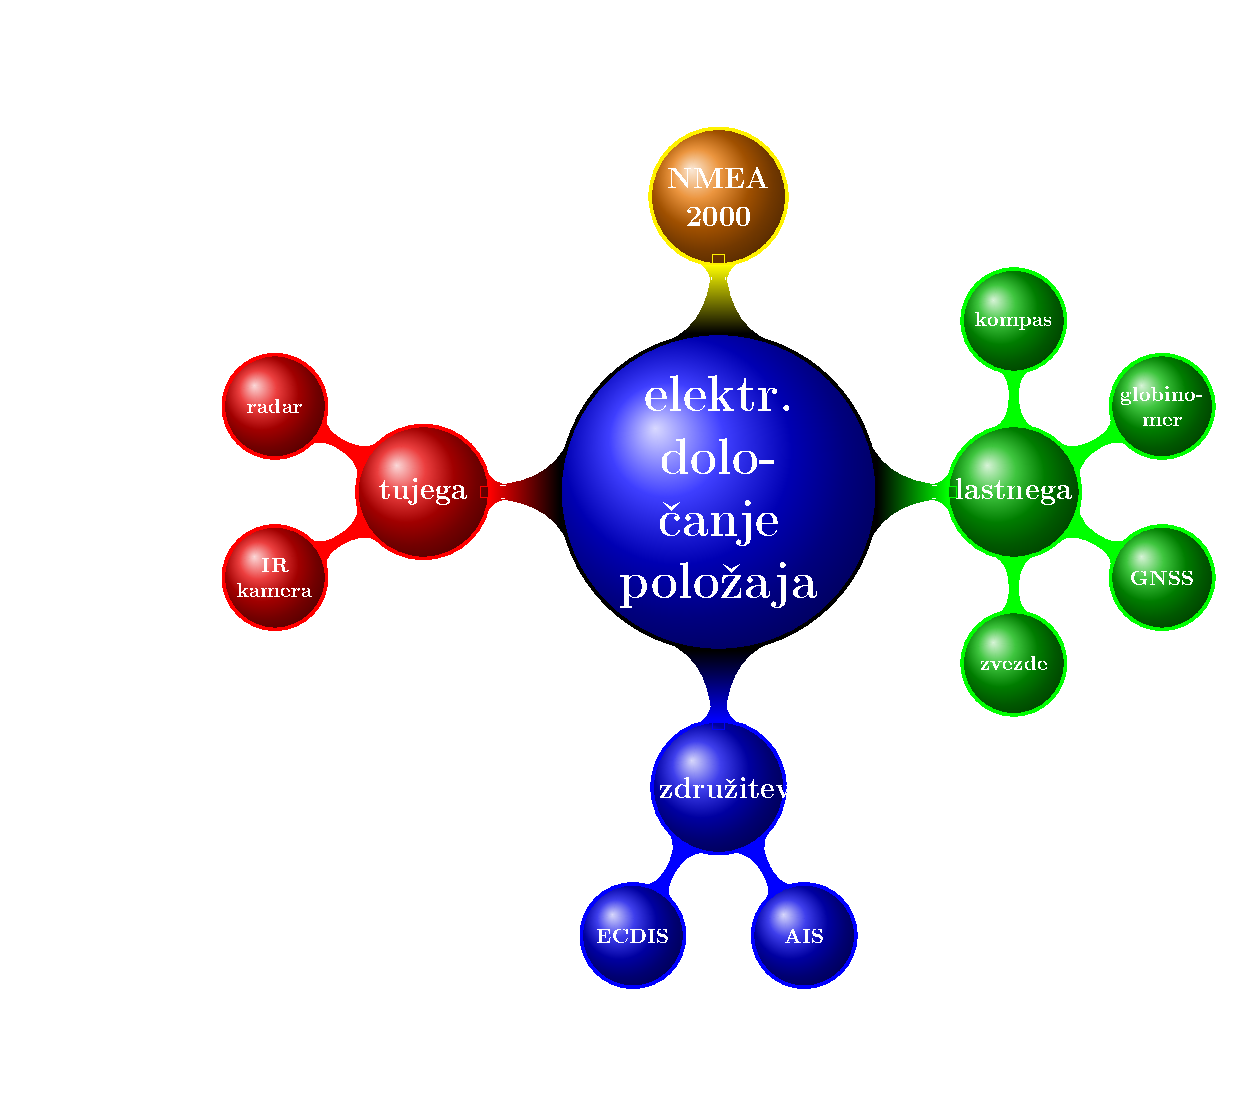
\includegraphics[height=9cm]{Predavanja/03_ElektrDolocPolozaja/figs/MiselniVzorec_ElDolPol.pdf}
	\caption{Miselni vzorec sodobnega določanja položaja na morju.}
	\label{fig:ShElDolP}
\end{figure}

\section{Seštevna navigacija in Fiksiranje položaja}
\label{sec:SestNavInFiksPoloz}

Med postopkom \textbf{seštevne navigacije} (ang. dead reckonning) instrumenti ali merijo spremembo položaja ali merijo hitrost, ki jo integrirajo. Vrednost integrala se dodaja prejšnjemu položaju, s čimer se izračuna trenutni položaj. Hitrost ali prepotovana razdalja se podajata vzdolž osi objekta, posebej se računata oba podatka, če ju določamo glede na okolico. Če se smer objektu spreminja, morajo biti za natančne določitve položaja časovni intervali vzorčenja kratki, preračuni so se opravljali ročno, danes jih izvajajo računalniki. Nekdaj uveljavljene mehanske merilnike hitrosti plovil (ang. log) nadomeščajo elektromagnetni log-i, globinomeri, ki vključujejo tudi merjenje hitrosti, laserski skenerji, spremembam v okolici sledeče kamere in radarji. Smer lahko merita kompas ali inercijski instrument (pospeškometer, merilnik nagiba). Tudi položaji Sonca, Meseca in zvezd na nebu lahko pomagajo določati smer, če natančno poznamo čase odčitavanj in približen položaj objekta. Z žiroskopi, ki merijo kotno hitrost, določamo spremembe smeri. Z integriranjem absolutnih in relativnih odčitkov smeri lahko določimo smer bolj točno in bolj odporno na motnje.     

INS je ..



\section{Osnovna načela delovanja hiperboličnih navigacijskih sistemov}
\label{sec:HiperbolSist}
% Always give a unique label
% and use \ref{<label>} for cross-references
% and \cite{<label>} for bibliographic references
% use \sectionmark{}
% to alter or adjust the section heading in the running head
\cite{monograph}.


\section{Automatic Identification System}
\label{sec:AIS}
Naloge AIS oddajnika so:
\begin{itemize}	
\item prikaz statičnih in dinamičnih podatkov: ime ladje, klicni znak, klicna digitalna številka MMSI, registracijska številka IMO, pristanišče, v katerega je ladja namenjena, stopnja nevarnosti tovora, ki ga ladja prevaža (lestvica International Maritime Dangerous Goods).;
\item oddajanje lastnih podatkov, sprejem in prikaz podatkov vseh ladij s podobno opremo AIS (vrsta A ali B), 
\item prikaz objektov ATON, plovil SAR (čoln, ladja, helikopter, letalo), SART oddajnikov in obalnih postaj;
nadzor, spremljanje in sledenje ladij ter izmenjava podatkov med ladjami, kakor tudi izmenjava podatkov s kopnim oz. obalnimi postajami;
možnost priključitve (Plug in) pilotskega modema za časa pilotaže in omogočanje razpolaganja z AIS podatki in informacijami lastne ladje ter drugih ladij in objektov.
\end{itemize}
\subsection{Subsection Heading}
\label{sec:2}
Your text goes here.

\begin{equation}
	\vec{a}\times\vec{b}=\vec{c}
\end{equation}

\subsubsection{Subsubsection Heading}
Your text goes here. Use the \LaTeX\ automatism for cross-references as
well as for your citations, see Sect.~\ref{sec:1}.

\paragraph{Paragraph Heading} %
Your text goes here.

\subparagraph{Subparagraph Heading.} Your text goes here.%
%
\index{paragraph}
% Use the \index{} command to code your index words
%
% For tables use
%
\begin{table}
	\centering
	\caption{Please write your table caption here}
	\label{tab:1}       % Give a unique label
	%
	% For LaTeX tables use
	%
	\begin{tabular}{lll}
		\hline\noalign{\smallskip}
		first & second & third  \\
		\noalign{\smallskip}\hline\noalign{\smallskip}
		number & number & number \\
		number & number & number \\
		\noalign{\smallskip}\hline
	\end{tabular}
\end{table}
%
%
% For figures use
%
\begin{figure}
	\centering
	% Use the relevant command for your figure-insertion program
	% to insert the figure file.
	% For example, with the option graphics use
	
\includegraphics[height=4cm]{figure}
	%
	% If not, use
	%\picplace{5cm}{2cm} % Give the correct figure height and width in cm
	%
	\caption{Please write your figure caption here}
	\label{fig:1}       % Give a unique label
\end{figure}
%
% For built-in environments use
%
\begin{theorem}
	Theorem text goes here.
\end{theorem}
%
% or
%
\begin{lemma}
	Lemma text goes here.
\end{lemma}
%
%
% Problems or Exercises should be sorted chapterwise
\section*{Problems}
\addcontentsline{toc}{section}{Problems}
%
% Use the following environment.
% Don't forget to label each problem;
% the label is needed for the solutions' environment
\begin{prob}
	\label{prob1}
	The problem\footnote{Footnote} is described here. The
	problem is described here. The problem is described here.
\end{prob}

\begin{prob}
	\label{prob2}
	\textbf{Problem Heading}\\
	(a) The first part of the problem is described here.\\
	(b) The second part of the problem is described here.
\end{prob}

\section{Pogoji za razširjanje elektromagnetnih signalov v zemeljski troposferi in v ionosferi}
\label{sec:1}
% Always give a unique label
% and use \ref{<label>} for cross-references
% and \cite{<label>} for bibliographic references
% use \sectionmark{}
% to alter or adjust the section heading in the running head
\cite{monograph}.



\section{Satelitska tehnologija, Kepplerjevi elementi}
\label{sec:1}
% Always give a unique label
% and use \ref{<label>} for cross-references
% and \cite{<label>} for bibliographic references
% use \sectionmark{}
% to alter or adjust the section heading in the running head
\cite{monograph}.

\section{Matematični pripomočki in triki}
\label{sec:1}
% Always give a unique label
% and use \ref{<label>} for cross-references
% and \cite{<label>} for bibliographic references
% use \sectionmark{}
% to alter or adjust the section heading in the running head
\cite{monograph}.


\section{Vpliv motenj na delovanje GNSS}
\label{sec:1}
% Always give a unique label
% and use \ref{<label>} for cross-references
% and \cite{<label>} for bibliographic references
% use \sectionmark{}
% to alter or adjust the section heading in the running head
\cite{monograph}.
Razlikovati moramo ozkopasovne in širokopasovne motilnike. Širokopasovni najbolj vplivajo na kodo iz katere sprejemnik določi lokacijo, ozkopasovni pa ne vplivajo na določitev lokacije, ampak kvarijo določanje Dopplerjevega pojava in s tem določitev smeri in hitrosti.

%

